% =====================================================================
%  preamble.tex —— 李思《Quantum Mechanics and Geometry》中文译注本 · 导言区
%  Lead 独占；译者只读，不得修改（需要新宏请在 reports/ 里提）
% =====================================================================
\usepackage[b5paper,top=21mm,bottom=21mm,left=19mm,right=19mm,headsep=5mm,footskip=9mm]{geometry}
\usepackage{amsmath,amssymb,mathrsfs,bm}
\usepackage{graphicx}
\usepackage{tikz}
\usetikzlibrary{arrows.meta,calc,decorations.pathmorphing}
\usepackage{xcolor}
\usepackage{booktabs,array,multirow,longtable,multicol}
\usepackage{enumitem}
\usepackage{fancyhdr}
\usepackage{caption}
\usepackage{tcolorbox}
\tcbuselibrary{most}
\usepackage{hyperref}
\hypersetup{colorlinks=true,linkcolor=black,citecolor=black,urlcolor=blue!45!black,
            bookmarksnumbered=true,
            pdftitle={量子力学与几何（李思 著，中文译注本）},
            pdfauthor={李思（Si Li）著}}

\setlength{\parindent}{2em}
\linespread{1.12}
\allowdisplaybreaks[2]
\setlength{\emergencystretch}{6em}
\tolerance=3000
\hbadness=10000

% 圈号 ①–⑳ 归入 CJK 字符类，否则会落到 Latin 字体而缺字（原书用 ①② 标注情形）
\xeCJKDeclareCharClass{CJK}{"2460 -> "2473}

% ---------- 页眉页脚 ----------
\pagestyle{fancy}
\fancyhf{}
\renewcommand{\headrulewidth}{0.3pt}
\fancyhead[LE]{\small\thepage}
\fancyhead[RE]{\small\leftmark}
\fancyhead[RO]{\small\thepage}
\fancyhead[LO]{\small\rightmark}
\renewcommand{\chaptermark}[1]{\markboth{\CTEXthechapter\quad #1}{}}
\renewcommand{\sectionmark}[1]{\markright{\thesection\quad #1}}

% ---------- 章节标题格式 ----------
\ctexset{
  chapter = {
    format = \centering\Large\bfseries,
    name = {第,章},
    number = \arabic{chapter},
    beforeskip = 18pt,
    afterskip = 22pt,
  },
  section = {
    format = \large\bfseries,
    beforeskip = 14pt,
    afterskip = 10pt,
  },
  subsection = {
    format = \normalsize\bfseries,
    beforeskip = 11pt,
    afterskip = 6pt,
  },
  subsubsection = {
    format = \normalsize\bfseries,
    beforeskip = 9pt,
    afterskip = 5pt,
  },
}

% ---------- 公式：原文无编号，一律不编号；个别带 (*) 的用 \tag{$*$} ----------

% ---------- 陈述环境：编号一律照抄原文（手工），不用自动计数器 ----------
% 用法： \begin{definition}{1.1.5} …… \end{definition}
\newcommand{\qmstmt}[2]{\par\medskip\noindent\textbf{#1~#2.}\ \ignorespaces}
\newenvironment{definition}[1]{\qmstmt{定义}{#1}}{\par\medskip}
\newenvironment{theorem}[1]{\qmstmt{定理}{#1}}{\par\medskip}
\newenvironment{lemma}[1]{\qmstmt{引理}{#1}}{\par\medskip}
\newenvironment{proposition}[1]{\qmstmt{命题}{#1}}{\par\medskip}
\newenvironment{corollary}[1]{\qmstmt{推论}{#1}}{\par\medskip}
\newenvironment{example}[1]{\qmstmt{例}{#1}}{\par\medskip}
\newenvironment{remark}[1]{\qmstmt{注}{#1}}{\par\medskip}
\newenvironment{assumption}[1]{\qmstmt{假设}{#1}}{\par\medskip}
\newenvironment{notation}[1]{\qmstmt{记号}{#1}}{\par\medskip}
\newenvironment{question}[1]{\qmstmt{问}{#1}}{\par\medskip}
\newenvironment{problem}[1]{\qmstmt{问题}{#1}}{\par\medskip}
\newenvironment{exercise}[1]{\qmstmt{练习}{#1}}{\par\medskip}
\newenvironment{conjecture}[1]{\qmstmt{猜想}{#1}}{\par\medskip}
\newenvironment{claim}[1]{\qmstmt{断言}{#1}}{\par\medskip}
\newenvironment{definition*}{\par\medskip\noindent\textbf{定义.}\ \ignorespaces}{\par\medskip}
\newenvironment{proposition*}{\par\medskip\noindent\textbf{命题.}\ \ignorespaces}{\par\medskip}
\newenvironment{example*}{\par\medskip\noindent\textbf{例.}\ \ignorespaces}{\par\medskip}
\newenvironment{remark*}{\par\medskip\noindent\textbf{注.}\ \ignorespaces}{\par\medskip}
% 证明（原文常作行内 “Proof:”）
\newenvironment{proof}[1][证明]{\par\medskip\noindent\textbf{#1.}\ \ignorespaces}{\hfill$\blacksquare$\par\medskip}
\newcommand{\proofless}{}

% ---------- 无题图（原文的 TikZ 图均无题注，按原页裁切嵌入）----------
% 用法： \begin{figure}[htbp]\centering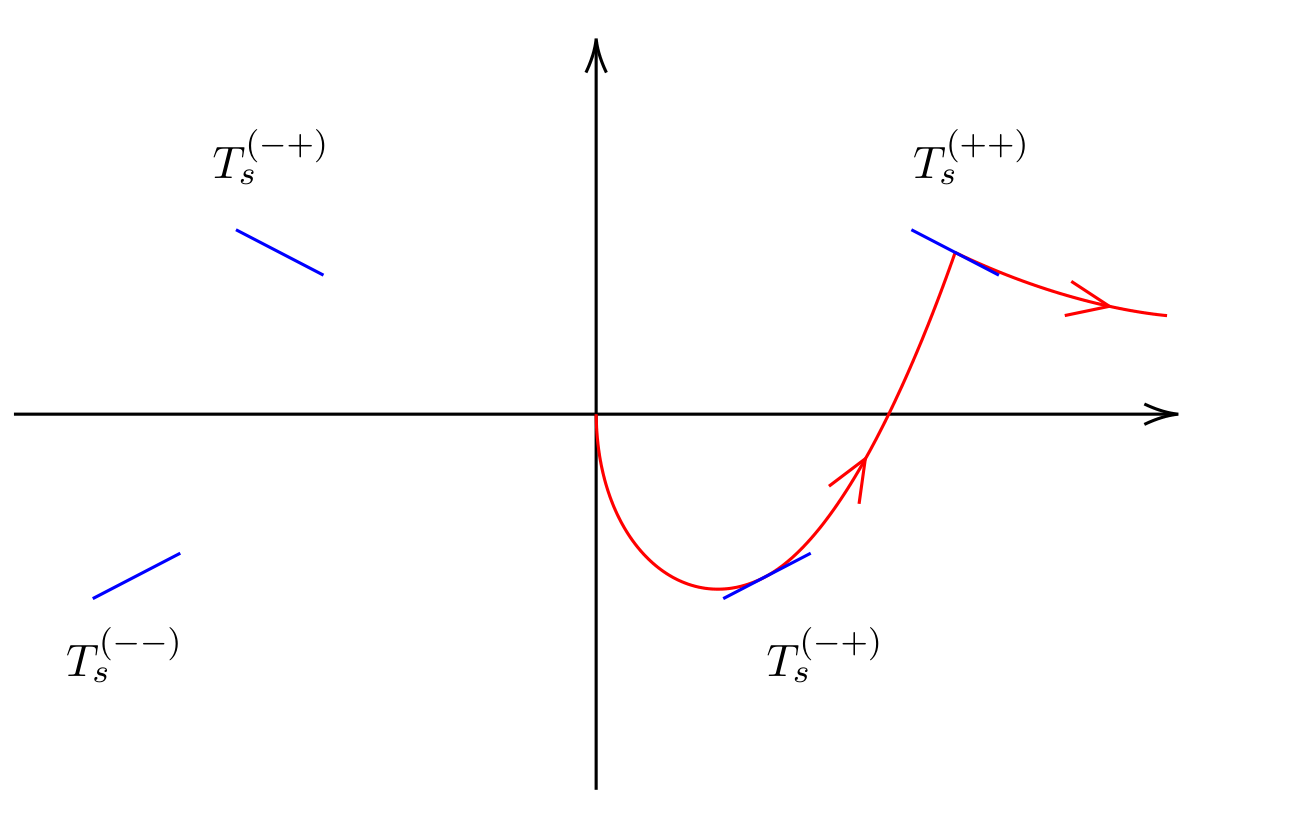
\includegraphics[width=.62\textwidth]{figures/fig_p137_a.png}\end{figure}
% 需要一行说明时用： \fignote{......（原书 p.136）}
\newcommand{\fignote}[1]{\par\smallskip\noindent{\centering\small #1\par}\smallskip}

% ---------- “本节重点” 与 “章末评注”（全局开关）----------
\newif\ifshowtakeaway       \showtakeawaytrue
\newif\ifshowchapterreview  \showchapterreviewtrue

\newtcolorbox{takeawaybox}{
  enhanced, colback=blue!4!white, colframe=blue!55!black,
  boxrule=0.4pt, arc=1.5pt, left=5pt, right=5pt, top=3pt, bottom=3pt,
  title={\small\bfseries 本节重点}, fonttitle=\small\bfseries,
  coltitle=white, colbacktitle=blue!55!black,
  attach boxed title to top left={xshift=4pt,yshift=-2pt},
}
\newtcolorbox{reviewbox}{
  enhanced, breakable, colback=orange!3!white, colframe=orange!65!black,
  boxrule=0.4pt, arc=1.5pt, left=6pt, right=6pt, top=4pt, bottom=4pt,
  title={\small\bfseries 本章回顾与评注}, fonttitle=\small\bfseries,
  coltitle=white, colbacktitle=orange!65!black,
  attach boxed title to top left={xshift=4pt,yshift=-2pt},
}
\newcommand{\takeaway}[1]{\ifshowtakeaway\begin{takeawaybox}\small #1\end{takeawaybox}\fi}
\newcommand{\chapterreview}[1]{\ifshowchapterreview\begin{reviewbox}\small #1\end{reviewbox}\fi}

% ---------- 常用记号 ----------
\newcommand{\R}{\mathbb{R}}
\newcommand{\C}{\mathbb{C}}
\newcommand{\Z}{\mathbb{Z}}
\newcommand{\Q}{\mathbb{Q}}
\newcommand{\N}{\mathbb{N}}
\newcommand{\CP}{\mathbb{C}\mathrm{P}}
\newcommand{\RP}{\mathbb{R}\mathrm{P}}
\newcommand{\HP}{\mathbb{H}\mathrm{P}}
\newcommand{\rd}{d}            % 微分 d
\newcommand{\ii}{i}            % 虚数单位 i
\newcommand{\ee}{e}            % 自然指数 e
\newcommand{\tr}{\operatorname{tr}}
\newcommand{\Tr}{\operatorname{Tr}}
\newcommand{\rank}{\operatorname{rank}}
\newcommand{\sgn}{\operatorname{sgn}}
\newcommand{\Real}{\operatorname{Re}}
\newcommand{\Imag}{\operatorname{Im}}
\newcommand{\id}{\mathrm{id}}
\newcommand{\Hom}{\operatorname{Hom}}
\newcommand{\End}{\operatorname{End}}
\newcommand{\Aut}{\operatorname{Aut}}
\newcommand{\Diff}{\operatorname{Diff}}
\newcommand{\Sym}{\operatorname{Sym}}
\newcommand{\Span}{\operatorname{span}}
\newcommand{\supp}{\operatorname{supp}}
\newcommand{\vol}{\operatorname{vol}}
\newcommand{\Loc}{\operatorname{Loc}}
\newcommand{\Op}{\operatorname{Op}}
\newcommand{\Res}{\operatorname{Res}}
\newcommand{\diag}{\operatorname{diag}}
\newcommand{\eps}{\varepsilon}
\newcommand{\sm}{\setminus}
% Dirac 记号
\newcommand{\bra}[1]{\langle #1|}
\newcommand{\ket}[1]{|#1\rangle}
\newcommand{\braket}[2]{\langle #1|#2\rangle}
\newcommand{\mel}[3]{\langle #1|#2|#3\rangle}
\newcommand{\expv}[1]{\langle #1\rangle}
\newcommand{\norm}[1]{\lVert #1\rVert}
\newcommand{\abs}[1]{\lvert #1\rvert}
\newcommand{\ip}[2]{\left\langle #1,#2\right\rangle}
\newcommand{\ps}{\psi}
\newcommand{\hs}{\hbar}
\newcommand{\pa}{\partial}
\newcommand{\nab}{\nabla}
\newcommand{\wt}[1]{\widetilde{#1}}
\newcommand{\wh}[1]{\widehat{#1}}
\newcommand{\ol}[1]{\overline{#1}}
\DeclareMathOperator*{\argmin}{arg\,min}
\DeclareMathOperator*{\argmax}{arg\,max}
\newcommand{\slim}{\operatorname{s-lim}}
\newcommand{\wlim}{\operatorname{w-lim}}
\newcommand{\Dom}{\operatorname{Dom}}
\newcommand{\Ran}{\operatorname{Ran}}
\newcommand{\Ker}{\operatorname{Ker}}

% ===== 译者批注（正文可见的小框）=====
\newcommand{\tutornote}[1]{%
  \par\smallskip\noindent
  \begin{tcolorbox}[colback=gray!7,colframe=gray!55,boxrule=0.4pt,arc=1pt,
    left=4pt,right=4pt,top=3pt,bottom=3pt,fontupper=\small,breakable]
  \textbf{译者批注}\quad #1%
  \end{tcolorbox}\smallskip}
